\documentclass[tikz,border=4pt]{standalone}
% Estilo común de los diagramas de bloques (se usa con \input en cada standalone)
\usepackage[defaultsans,scale=0.92]{lato}
\usepackage{libertinust1math}
\usepackage{xcolor,amsmath}
\usepackage{tikz}
\usetikzlibrary{positioning,arrows.meta,calc,shapes.geometric}
\usepackage{../../notacion}
\definecolor{ctrlazul}{HTML}{1E5AA8}\definecolor{ctrlnoche}{HTML}{14213D}
\definecolor{ctrlcoral}{HTML}{D1495B}\definecolor{ctrlverde}{HTML}{2A9D8F}
\definecolor{ctrlambar}{HTML}{E09F3E}\definecolor{ctrlgris}{HTML}{5C677D}
\definecolor{ctrlvioleta}{HTML}{6C4AB6}\definecolor{ctrlteal}{HTML}{0F7173}
\tikzset{
  >={Stealth[length=2.4mm]}, every node/.style={font=\small},
  bloque/.style={draw=ctrlnoche,fill=ctrlazul!7,thick,rounded corners=1.5pt,minimum height=9mm,minimum width=13mm,inner sep=4pt},
  suma/.style={draw=ctrlnoche,thick,circle,inner sep=0pt,minimum size=6mm},
  senal/.style={->,thick,draw=ctrlnoche},
  rot/.style={font=\footnotesize,text=ctrlgris},
}

\begin{document}
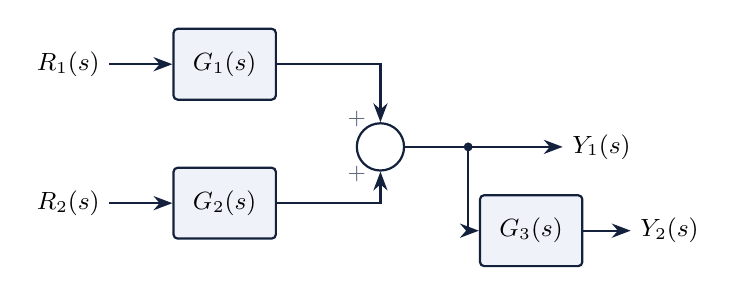
\begin{tikzpicture}[node distance=8mm]
  \node (r1) {$R_1(s)$}; \node[bloque,right=of r1] (g1) {$G_1(s)$};
  \node[below=12mm of r1] (r2) {$R_2(s)$}; \node[bloque,right=of r2] (g2) {$G_2(s)$};
  \node[suma,right=10mm of g1,yshift=-10.5mm] (S) {};
  \coordinate[right=8mm of S] (n); \fill[ctrlnoche] (n) circle (1.6pt);
  \node[right=12mm of n] (y1) {$Y_1(s)$};
  \node[bloque,below=6mm of n,xshift=8mm] (g3) {$G_3(s)$}; \node[right=6mm of g3] (y2) {$Y_2(s)$};
  \draw[senal] (r1)--(g1); \draw[senal] (r2)--(g2);
  \draw[senal] (g1)-|(S); \draw[senal] (g2)-|(S);
  \node[rot] at ($(S)+(-3mm,3.5mm)$) {$+$}; \node[rot] at ($(S)+(-3mm,-3.5mm)$) {$+$};
  \draw[thick,draw=ctrlnoche] (S)--(n); \draw[senal] (n)--(y1); \draw[senal] (n)|-(g3); \draw[senal] (g3)--(y2);
\end{tikzpicture}
\end{document}
